\section{Introducción}
El problema que se nos pide resolver consiste en la elaboración de distintos algoritmos que indiquen a nuestro avatar cuál es la mejor acción posible para completar los requisitos de los distintos tipos de mapas de la forma menos costosa o simplemente aguantar el mayor tiempo posible sin morir. Los requisitos anteriormente mencionados pueden ser tan simples como buscar una puerta en el mapa y alcanzarla en el menor número de acciones, o encontrar 10 diamantes antes de buscar la puerta, tratar de evitar a uno o varios enemigos durante 2000ticks o en el último caso todo lo anterior.

El código está preparado para cambiar entre los distintos comportamientos basándose en los datos del mapa, por ejemplo, los comportamientos reactivos simple y compuesto sólo funcionan si el mapa presenta enemigos pero no presenta diamantes, para el caso de que ambos elementos estén se enceuntren en el mapa se procederá con el comportamiento reactivo deliberativo. Para esto se han introducido diversas variables que durante la inicialización cambian de valor para controlar la ejecución correcta de cada comportamiento:

\begin{itemize}
\item \textbf{gemas} Se trata de un entero inicialmente a 0, durante la inicialización se comprueba mediante el método getResourcePositions si el array que se devuelve es nulo, indicando que el mapa no presenta gemas, la variable pasa a 10, como el comportamiento buscan una puerta siempre que el número de gemas sea igual o mayor que 10 buscará la puerta directamente.
\item \textbf{sobrevivir} Variable booleana que pasa a ser true siempre que el array devuelto por el método getNPCPositions no sea nulo, su uso se combina con el de la siguiente variable para detectar si nos encontramos en un mapa reactivo o reactivo deliberativo, en caso de que no existan gemas en el mapa sobrevivir siempre será true, de forma que el avatar estará buscando siempre que se encuentre en peligro la casilla con menor calor a su disponibilidad, la medición del peligro se explica en el punto 4.
\item \textbf{gemas$\_$sobrevivir} Esta variable pasa a ser verdadero si y sólo si en el mapa hay enemigos y gemas, en este caso, se matiende a true durante toda la ejecución del programa, esto es así ya que se ha decidido usar la variable sobrevivir para detectar en el mapa reactivo deliverativo si nuestro avatar se encuentra en peligro. Si se alcanza una casilla con peligro 0, sobrevivir vuelve a ser false.
\end{itemize}

Se han asumido las siguientes propiedades de cada mapa, en caso de que no se cumpliesen los diversos comportamientos actuarían de forma extraña:
\begin{itemize}
	\item Todas las gemas y el portal son acesibles, es decir no existe la posibilidad que se genere un portal rodeado de muros.
	\item Sólo hay un portal en el mapa, de forma que en caso de un mapa con varios sólo se buscará el más cercano.
	\item Todos los enemigos se mueven de la misma forma que los escorpiones y no existe ningún otro tipo de peligro.
\end{itemize}

\section{Comportamiento Deliberativo Simple}
En este caso se nos presenta un mapa con diversos muros y una única puerta. Se trata de un problema de búsqueda  del camino más corto desde un punto A a otro B. Para esto se ha decidido implementar un algoritmo de búsqueda A-estrella, empleando una modificación de la clase nodo de GVGAI. Para la valoración se ha decidido usar la distancia Manhattan del nodo en concreto al portal, sumando 1 en caso de que fuese necesario girarse y sumando el coste de su nodo padre, de esta forma cuanto menor sea la valoración del nodo mejor es, puesto que menos pasos vamos a necesitar para alcanzar la puerta, la generación de los nodos hijos es siempre comprobando las casillas superior, inferior, derecha e izquierda del nodo padre, en primer lugar nos aseguramos de que no se trate de un muro, en cuyo caso descartamos este movimiento al no ser posible. Siempre que se llama al método actuar se introduce en el array Abierto de nodos uno creado con las coordenadas de la casilla en la que se encuentra actualmente el avatar y con valoración igual a la distancia manhattan entre el avatar y el portal.

Para el mapa 6 este algoritmo encuentra un camino de 28 ticks en el tiempo aproximado de 10 milisegundos, realizando un total de 90 evaluaciones antes de encontrar el nodo que comparte las coordenadas del portal, tras esto se recorren sus nodos padres hasta llegar a un nodo con acción Nil, esto nos indica que se trata del primer nodo que se introdujo en abiertos luego su hijo contiene la acción a realizar. Repetiremos este proceso hasta alcanzar la puerta, con cada ejecución consecutiva el tiempo de que tarda en encontrar la puerte se reduce y el número de nodos explorados también.

\subsection{Selección de A-estrella}
Se ha decidido implementar como algoritmo de búsqueda A* debido a que se rechazaron las otras opciones, por los siguientes motivos:

\textbf{Djisktra} Se asumió que al tratarse de un algoritmo que calcula la distancia de un nodo origen al resto de los nodos y el problema que estaos tratando de resolver presenta un gran número de nodos, Djisktra no podría porporcionar una solución en menos de 40ms.

\textbf{Greedy} Al tratarse esencialmente de un algoritmo menos completo que A*, debido a que sólo usa la heurística para valorar los nodos, no tiene en cuenta el camino ya recorrido, fué descartado también por A-estrella.

Al implementar A-estrella y ver que porporcionaba buenos resultados en un tiempo más que aceptable (10 milisegundos) se decidió continuar con el resto de comportamientos.

\section{Comportamiento Deliberativo Compuesto}
En este caso se nos presenta buscar 10 gemas en un mapa con un número de gemas igual o superior, y luego salir por la puerta. Se trata del problema del viajante de comercio, Para este se ha decidido crear una nueva lista con las coordenadas de los diamantes que se han decidido recolectar.

Durante la inicialización del programa se elabora la lista mencionada anteriormente, primero buscamos la pareja de diamantes más cercanos, guardando ambos en el vector, tras esto buscamos los diamantes que se encuentren más cerca del principio y final del vector, comparamos las distancias de estos dos diamantes y nos volvemos a quedar la mas corta, tras esto lo añadimos al inicio o fondo del vector en función de a cuál de ellos fuese el más cercano en primer lugar. Repetiremos este proceso con el nuevo inicio o final hasta obtener un vector de 10 coordenadas. Durante la elaboración de la lista no se tienen encuenta el portal ni la posición avatar, se ha decidido implementar sin tener encuenta ninguna de las dos ya el algoritmo en su estado actual proporciona un redimiento aceptable.

Tras obtener este vector se procede con un algoritmo A-estrella idéntico al anterior, con la única diferencia que las coordenadas objetivo corresponden con las del array de diamantes, una vez se ha obtenido un diamante se pasa al siguiente y cuando se han obtenido los 10 se busca la puerta.

Para el mapa 7 el algoritmo encuentra un camino en 100 ticks, se reconoce que este número de pasos no se acerca al óptimo pero se decidió mantener y no buscar otro algoritmo de elaboración de una lista de coordenadas ya que se sospecha que el motivo se encuentra en el A estrella implementado aunque no se ha podido discernir la causa exacta, sin embargo debido a los buenos resultados que presenta con el comportamiento deliberativo simple se optó por conservar auqnue esto implicase que la búsqueda de un camino hacia cada diamante no fuese la óptima.

\subsection{Otros algoritmos considerados}
En primer lugar se planteó la opción de usar A*, inicialmente la lista no consistía únicamente do coordenadas de diamantes, sino que incluía la posición inicial del avatar y al final la del portal, se planteó que se podría consisderar la lsita como un nodo, siendo el nodo inicial la lista con las coordenadas del avatar, y generar sus hijos guardándolos en un vector de abirtos y puntuando las nuevas listas en función de la distancia manhattan de el primer elemento al segundo, del segundo al tercero, etc... Se tomaría la lista con menor coste y se volverían a generar sus hijos, continuando de esta forma hasta obtener una lista con 12 elemento (siendo el portal siempre el último), tras implementarse se descubrió que el proceso era considerablemente lento y no se podía obtener una lista en el tiempo máximo permitido debido a que se exploraban demasiados nodos, se consideró que quizás dividiendo el coste de los caminos entre el número de elementos reduciría el número de nodos explorados, pero entonces con la lista obtenida por el algoritmo, se tardaban 113 ticks en completar el mapa 6, finalmente la idea de tratar de usar A* se descartó.

\section{Comportamiento Reactivo Simple y Compuesto}
Debido a que se ha implementado el mismo comportamiento para ambos se han recogido las decisiones juntas, aunque la mayoría de las veces los escorpiones no llegan a matar al jugador, al moverse aleatoriamente, en ocasiones se da la situación en la que lo acorralan en una esquina y ambos le impiden salir. Se planteó la idea de que en caso de que se diese esta situación, el avatar tratase de acortar entre ambos escorpiones, sin embargo, como esto ocurre casi exclusivamente en esquinas acortar entre ambos implicaría moverse haciendo zigaz, y como se ha comporbado en el comportamiento deliberativo esto es extremadamanete costoso y daría incluso más tiempo a los escorpiones a alcanzar al jugador, de forma que se descartó esta solución. Se decidió hacer la diferencia de calor entre los círculos exteriores e interiores más evidente de forma que en caso de estar en el rango de dos escorpiones prefiera acercarse a uno si con esto consigue escapar del otro, esto se ha implementeado así ya que al moverse aleatoriamente las posibilidades de que uno solo avanza hacia el avatar son menores que cuando se trata de dos enemigos.

Para el comportamiento reactivo simple nos encontramos en un mapa con un único enemigo que puede moverse en diagonal, al contrario que el jugador, el objetivo es sobrevivir 2000 ticks, para ello se ha elaborado un mapa de calor como el del siguiente diagrama. El cálculo de este área se hace siempre desde el enemigo, siempre que se llama al método actuar se comprueba si la casilla del avatar tiene algún nivel de peligro, en caso de que este sea mayor que 0, probamos a buscar la casilla superior, inferior, derecha o izquierda que menos peligro tenga y devolvemos la actuación para dirigirnos hacia ella, debido ha cómo se realiza el cálculo de calor una casilla puede tener el calor considerabalemente alto si se encuentra en el rango de ambos enemigos, pero nunca lo suficientemente alto como para que el avatar cosidere beneficioso acercarse a ninguno de los dos, en anteriores implmentanciones se cometió este error, causando que en caso de ser rodeado, el avatar huyese hacia un escorpión y en la amyoría de ocasiones muriese.

\begin{figure}[H]
    \caption{Mapa de calor para los escorpiones}
    \centering
	 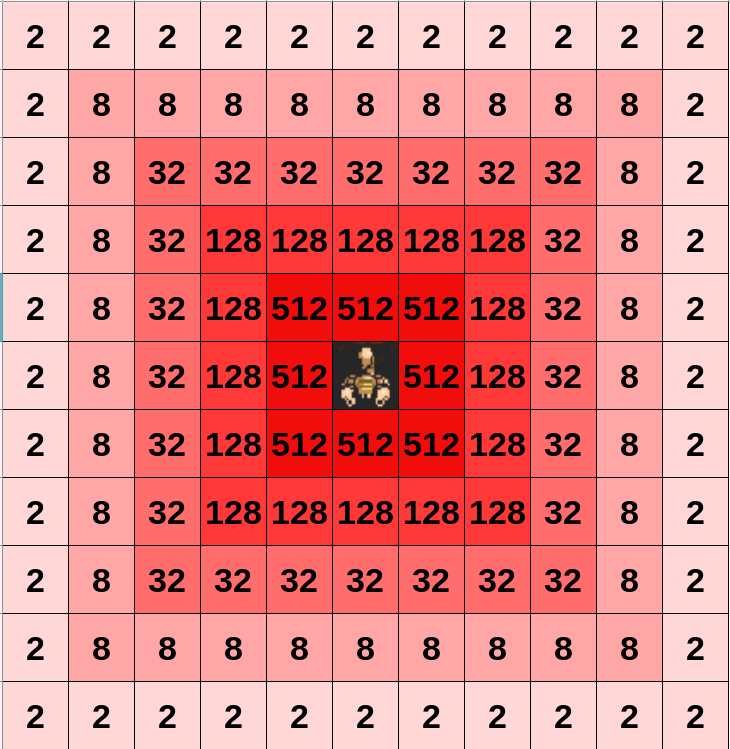
\includegraphics[scale=0.25]{Escorpiones.png}
    \label{fig:label}
\end{figure}

Además debido a que con únicamente esto, el avatar moría varias veces ya que se auto encerraba así mismo en una esquina o pared, se pensó en introducir peligro en las casillas con muros cercanos, siendo el calor estas 2, y el calor de las casillas cercanas a ellas 1, con la intención de que el avatar trate de evitarlos pero aún así prefiera los muros a acercarse al escorpión. El calor de los muros se calcula desde una segunda función alternativa tomando como origen la posición del avatar y comprobando primero las casillas a 1 paso de distancia y en caso de que no se tatasen de muros comporbar las casilla situadas a 2 pasos de distancia. Se consideró que de esta forma se aseguraría que nuestro avatar tendría un buen espacio de separación en caso de no verse activamente perseguido por los escorpiones, al final fué descartada debido a que tras varios intentos realizados el avatar moría más veces con la implementación que considerada las casillas adyacentes a las casillas junto a los muros peligrosas, se planteó también la idea de que el mapa de calor era excesivamente grande causando que el avatar tratase de huir desde mucho antes y acabase arrincoándodes, los resultado obtenidos para el mapa 2 fueron mucho peores de forma que se decidió mantener un mapa de calor de 11x11.

Otra alternativa fue la de tratar de buscar el centro del mapa siempre que el avatar no se encontrase en peligro, también fue descartada porque no se veía ningun tipo de mejora y se asumió que el avatar moriría en ciertas ocasiones si daba la casualidad que los escorpiones lo obligaban a retroceder hacia una esquina.

\section{Comportamiendo Reactivo-Deliberativo}
Para el comportamiento ractivo deliberativo se han introducido una única variable que detecta si en el mapa hay gemas y enemigos, entonces se trata de un mapa reactivo-deliberativo. Para este tipo de mapas se ha decidido que el avatar actúe exactamente igual que el comportamiento deliberativo compuesto siempre que el peligro en el que se encuentre sea 0, en caso de que sea mayor que 0 trata de alejarse del escorpión y escapar. Se podría haber planteado una fucnión para recalcular el orden en el que recolectar las gemas si el protagonista se había visto obligado a huir, pero fue descartada ya que se consideró que la elaboración de una nueva lista y además la búsqueda de su primer elemento podría causar un exceso de tiempo que obligase a devolver la acción nil.

En este último mapa el número de ticks que se requieren para completarlo es aleatorio, ya que el escorpión puede bloquear de forma indefinida la puerta o un diamante obligando al avatar a retirarse constantemente, se planteó como solución la opción de reducir el área de peligro del avatar pero se descartó ya que ocasionaría que el avatar se pusiese en peligro sin forma de huir, de manera que se optó por una aproximación más segura pero más lenta, manteniendo el calor del escorpión pero ignorando el del las paredes.

\section{Resultados finales y otras pruebas realizadas}

\begin{center}
\begin{tabular}{| c | c | c | c | c |}
 \hline
	28 ticks & 100 ticks & 80$\%$ de supervivencia & 60$\%$ de supervivencia & entre 120 y 300 iteraciones \\
 \hline
\end{tabular}
\end{center}
\indent En relación a los mapas  5, 6 y 9 se considera que se han obtenido resultados más que aceptable, aunque, las tasas de supervivencia de los mapas 8 y 7 son considerabalmente más bajas de las esperadas, hay que tener en cuenta que el porcentaje se ha tomado con la realización de tan solo 10 pruebas, por lo que es bastante probable que se trate de un estudio muy poco fiable, no se han realizado un número mayor de prueba debido a la gran cantidad de tiempo que consumiría, pero se ha querido reflejar lo que puede esperarse cuando se ejecute el código.
